\documentclass{article}
\usepackage[english]{babel}
\usepackage[utf8]{inputenc}
\usepackage{fancyhdr}
\usepackage{geometry}
\usepackage{enumitem}
\usepackage{amsmath, amssymb}
\usepackage{graphicx}
\usepackage{float}
\usepackage{gensymb}
\usepackage[thinc]{esdiff}

\geometry{letterpaper, portrait, margin=1in}
\graphicspath{ {images/} }
\pagestyle{fancy}
\fancyhf{}
\lhead{Keerthik Muruganandam}
\rhead{September 13th, 2021 Written Work 1}

\begin{document}

\begin{enumerate}[label=\textbf{(1.\arabic*)}]

\item Match each of the differential equations with its direction field below. Give a brief, unambiguous explanation for your choice.
\begin{center}
(a) $y^\prime = x^2	-y^2$\qquad\qquad\qquad\qquad\qquad\qquad\qquad (b) $y^\prime - y = 1$
\begin{figure}[H]
\centering
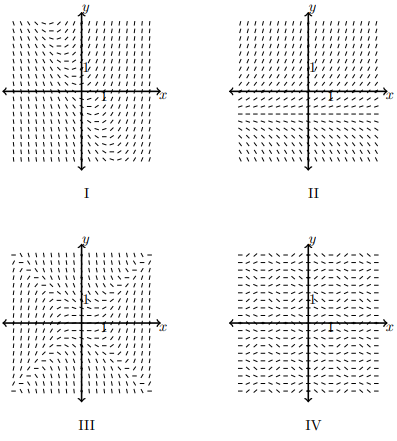
\includegraphics[scale=0.75]{problem1}
\end{figure}
\end{center}

\begin{enumerate}
\item First, let us consider the point $(1,-2)$. According to the differential equation, the derivative at $(1,-2)$ should be
\begin{align*}
y^\prime &= x^2-y^2\\
&= 1^2-2^2\\
&= -3
\end{align*}
The only direction field with a slope resembling $-3$ at $(1,-2)$ given that three slope lines is equal to one unit is III.

\item As you can clearly see, this is an autonomous differential equation. The only autonomous direction field is II. Therefore, the matching direction field is II.
\end{enumerate}

\newpage

\item \textbf{Newton's Law of Cooling} states that the rate of cooling of an object is proportional to the temperature difference between the object and its surroundings, provided that the difference is not too large.\\
At 10:00 AM, your dad makes you a cup of coffee that is $212\degree F$. The temperature of your house is fixed at $68\degree F$.
\begin{enumerate}
\item Write a DE that expresses the Law of Cooling for this scenario. Use $k$ as constant of proportionality.
\item Use Euler's Method with a step size of 2 minutes to estimate temperature of your chai at 10:02 AM.
\item If the chai was $190\degree F$ as 10:02 AM, estimate $k$ using (a) and (b)
\end{enumerate}
\vspace{10pt}
\begin{enumerate}
\item Let $t$ be time, $T$ be the temperature of the chai, and $T_r$ be the temperature of the room. The following differential equation expresses Newton's Law of Cooling in this situation.
\[\diff{T}{t} = k(T-T_r)\]
\item Euler's Method can be simplified in this case, considering that there is only one step. The temperature of the chai can be given as 
\[y_1=y_0+2\left(\diff{T}{t}\right)\]
The derivative is calculated as 
\begin{align*}
\diff{T}{t} &= k(T-T_r)\\
&= k(212\degree F - 68\degree F)\\
&= 144k
\end{align*}
Thus, the estimated temperature is $212\degree F + 292k$.
\item If the actual temperature was $190\degree F$ at 10:02 AM, we can set up a simple equation:
\[190 = 212 +292k\]
Solving as so,
\begin{align*}
212 +292k&= 190\\
292k &= -22\\
k &= \frac{-22}{292} = -\frac{11}{146}
\end{align*}
We can conclude $k$ is approximately $-\dfrac{11}{146}$.
\end{enumerate}

\newpage

\item For each of the following, briefly explain your answers.
\begin{enumerate}
\item Verify that all members of the family $y=\dfrac{1}{C-x}$ are solutions of the equation $y^\prime = y^2$.
\item What is a solution for the DE $y^\prime = y^2$ that is not a part of the family in part (a).
\item Find a solution for the initial value problem, $y^\prime =y^2$, $y(2)=3$.
\end{enumerate}

\begin{enumerate}
\item To verify this, just square and differentiate $y$ to show that they are equal.
\begin{align*}
\diff{y}{x} \left(\frac{1}{C-x}\right) &= \diff{y}{x} \left(({C-x})^{-1}\right)\\
&= (C-x)^{-2}\\
&= \frac{1}{(C-x)^{2}}
\end{align*}
The square of y is $\left(\dfrac{1}{C-x}\right)^2 = \dfrac{1}{(C-x)^2}$. All members of the family $y=\dfrac{1}{C-x}$ are solutions of the equation $y^\prime = y^2$. 
\item One simple solution to the DE is $y=0$. Its derivative is 0 and its square is 0 while also not being a part of the family in part (a).
\item Input the values of the initial-value into the equation in part (a) and solve for C.
\begin{align*}
3 &= \frac{1}{C-2}\\
3(C-2) &= 1\\
3C-6 &= 1\\
3C &= 7\\
C &= \frac{7}{3}
\end{align*}
The solution is $y=\dfrac{1}{\dfrac{7}{3}-x}$.
\end{enumerate}

\newpage

\item \textbf{Professional Problem Skills Practice.} Hand draw a rough sketch of the direction field for the autonomous differential equation
\[y^\prime = f(y),\]
where the graph of f is shown below. Be sure to carefully label the important features of your plot and format it like a figure that would be included in a full problem, including necessary labels. Use one or two sentences after the figure to show that you know how to correctly reference your figure in the body of the problem.
\begin{figure}[H]
\centering
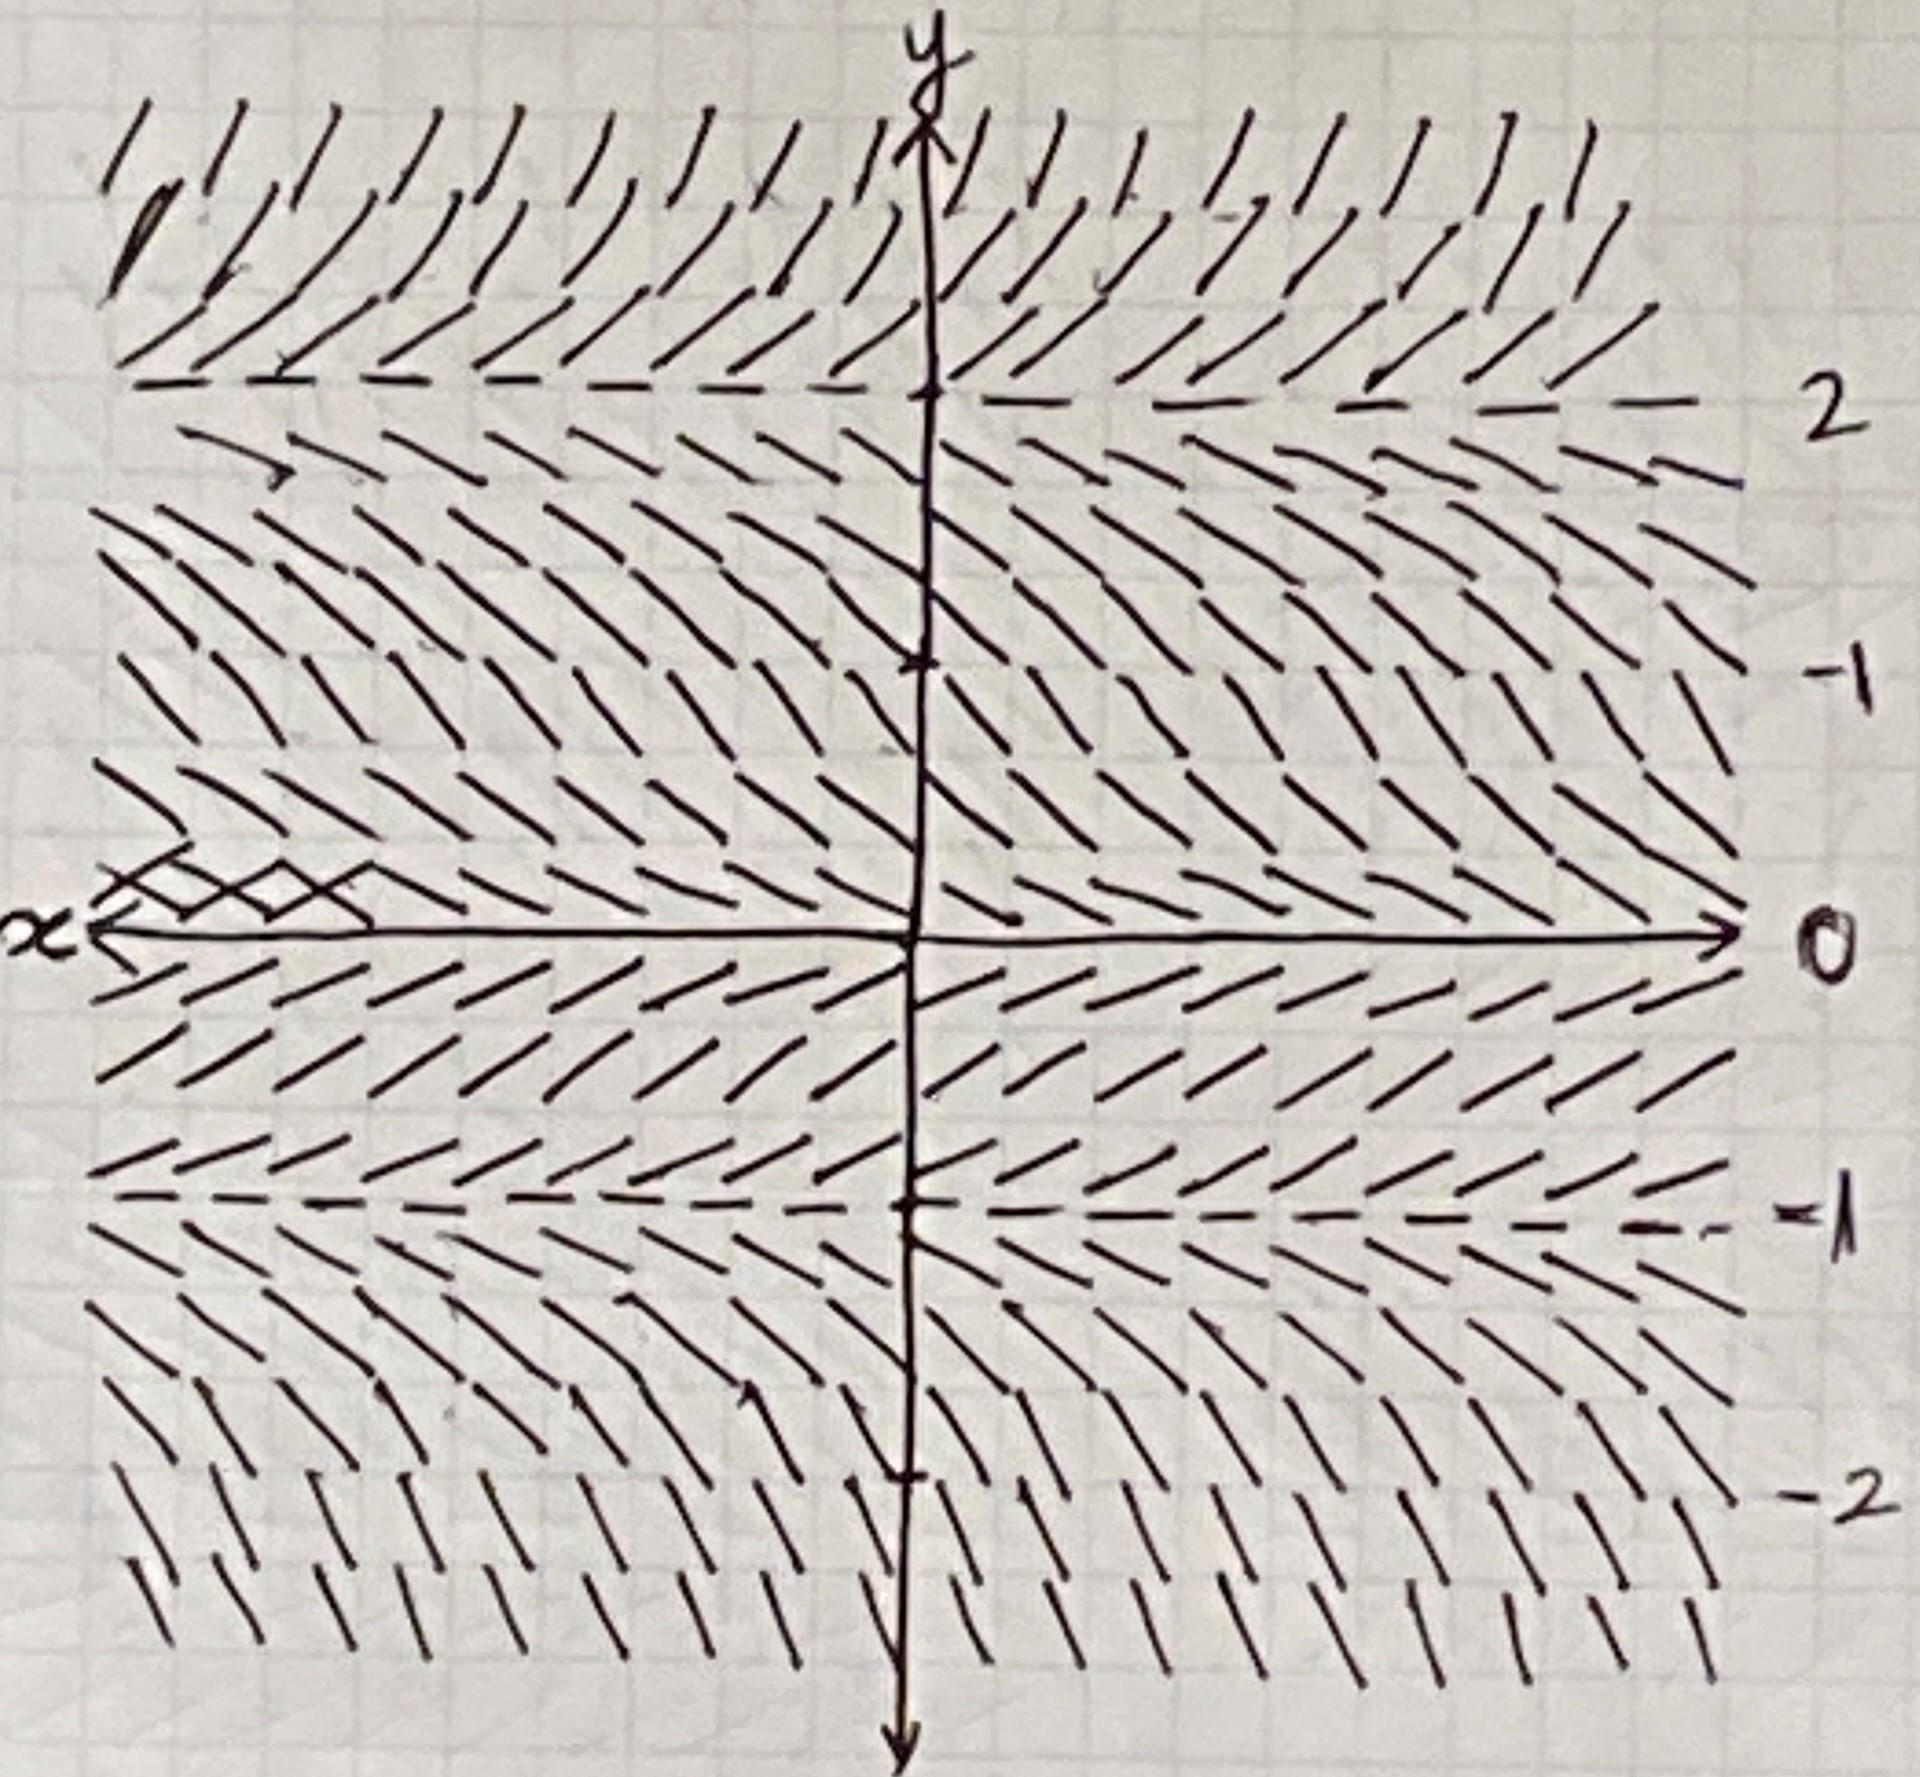
\includegraphics[scale=0.1]{ppp}
\caption{Direction Field}
\end{figure}
Figure 1 depicts the direction field for the autonomous differential equation $y^\prime = f(y)$. Notice that the slope of the lines only is changes is the value of $y$ changes, not when $x$ changes.

\end{enumerate}



\end{document}

